\documentclass[twoside,openright,a4paper,11pt,french]{article}
\usepackage[utf8]{inputenc}
\usepackage[french]{babel}
\usepackage[T1]{fontenc}
\usepackage{emptypage}

% Utilisation d'url
\usepackage{url}
\urlstyle{sf}

% Utilisation d'images, stockées dans le répertoire ./pics/
\usepackage{graphicx}
\graphicspath{pics/}

% Définition des marges
\usepackage{geometry}
\geometry{
  left=25mm,
  right=25mm,
  top=25mm,
  bottom=25mm,
  foot=15mm
}

\begin{document}

\pagestyle{plain}

% La page de garde
\thispagestyle{empty}

\begin{center}
       \noindent
       
\includegraphics[height=2.5cm]{./pics/uds.eps}       
       
       \vfill\vfill

    {\large \textsc{Licence 3 de Sciences, mention Informatique}}

    \bigskip\bigskip

    {\large \textsc{Réseaux et Protocoles}}

    \vfill\vfill

% Titre du document
    {\huge \sc
      \begin{center}
		Modèle de document\\pour un rapport d'étude
      \end{center}}

    \vfill\vfill

    {\large Présenté par}

\medskip

% Identité des auteurs
    {\large Julien \textsc{Montavont}}

% Contact mail
    {\small \url{montavont@unistra.fr}}

\bigskip

\end{center}



% La table des matières
\parskip=0pt
\tableofcontents


\section{Introduction}
\label{sec:intro}

% Daniel intro

A la fin des années 1960 il y eu une forte demande de la part des universités et centres de recherche aux Etats-Unis pour la création d'un réseau permettant d'une part, d'interconnecter les différentes structures afin de partager les informations et d'autre part, de faire des expérimentations sur les réseaux. 
C'est dans le but de faire ce réseau que l'ARPA a créé l'ARPANET qui est l'ancêtre d'internet. En effet, c'est à partir des principes de ce réseau qu'a été créé internet. L'ARPA (Advanced Research Project Agency ) est une agence de recherche créée par le département américain de la défense en 1957 afin de développer de nouvelles technologies à usage militaire. L'ARPA a mis en place en 1969 le premier réseau mondial qui a été appelé ARPANET ( Advanced Research Project Agency NETwork ). Ce réseau a été conçu de façon a ne pas dépendre d'un centre névralgique qui aurait pu être détruit en cas d'attaque nucléaire. Ce réseau a été constitué comme une toile reliants plusieurs serveurs. Chaque serveur est un noeud et peut stocker, traiter ou servir de relais. Ainsi, il existe plusieurs chemins pour accéder à un noeud et lorsqu'un noeud est hors service, il est toujours possible de rejoindre le noeud destinataire en passant par un autre chemin. Avant ARPANET, la communication réseau était également basée sur la communication par circuit électrique dont les  informations étaient envoyées en continue dans un seul morceau. Ce réseau est  le premier qui fonctionne sur la base de paquets. L.e principe de communication par paquet est de découper l'information à transmettre en de plus petits paquets qui peuvent chacun prendre un chemin différent pour arriver à destination.
Ce réseau se développa est il compta 23 noeuds en 1971 et en 1977 il en compta 111. Afin d'uniformiser ce réseau, Vint Cerf et Bob Kahn on introduit la première version du protocol TCP.
Historiquement, les protocoles IP constituaient la partie du protocole TCP qui s'occupe de la transmission en mode sans connexion. La transmission en mode sans connexion est une transmission de donnée dans laquelle chaque paquet contient l'adresse de destination. Ceci permet une transmission  du paquet sans que les deux hôtes soient obligés d'établir une connexion auparavant. Cette version est ce qu'on aurait pu nommer l'IPV1 et elle est documentée dans la RFC 675. Cette version fut modifiée et publiée en 1977. Elle correspond à la deuxième version de TCP (IPV2).
Initialement, le protocole TCP avait deux fonctions. ( as a host level end to end protocol, and to serve as an internet packaging and routing protocol. These two things should be provided in a layered and modular way. I suggest that a new distinct internetwork protocol is needed, and that TCP be used strictly as a host level end to end protocol.”) Premièrement, il devait permettre une transmission fiable d'informations entre deux hôtes. Il devait également servir en tant que protocole de routage et de packaging. Cependant, pour être cohérant avec le modèle en couche, qui différencie la fiabilité (couche transport) et le routage (couche réseau), il fut décidé en 1978 de diviser le protocole TCP. Le protocole TCP ne s'occupe maintenant plus que de la partie transport. La partie réseau a été prise en charge par les protocoles IP.
C'est finalement le 1er janvier 1983 que l'ARPANET adopte les protocoles TCP/IP et donc l'IPV4. 


% ------------------------------------------------

La technique de classe d'adressage IP ( classful network ) est une méthode utilisée de 1981 à 1993 pour allouer des adresses IPV4. Il a été défini en 1981 qu'une adresse IP est divisée en deux parties : une partie qui sert à identifier le réseau et une partie qui sert à identifier une interface sur ce réseau.
Dans cette méthode une adresse IP est divisée en 5 plages d'adresses IP et sont appelées classes. Ils sont organisés comme dans le tableau ci-dessous  :

\includegraphics{./pics/tableau.eps}


Chaque classe a un certain nombre d'octets servant à identifier le réseau. Une adresse IP de classe A à un identificateur de réseau sur 1 seul octet. Une adresse IP de classe B sur 2 octet et une de classe C sur 3 octets. Les adresses IP de classe D et E correspondent à des adresses IP particulières.
Les réseaux des différentes classes utilisent un certain nombre d'octets pour identifier le réseau. Ils ont donc un nombre différent d'octets restants qu'ils peuvent donner à des interfaces. 
Pour déterminer à quelle classe appartient une adresse IP il suffit de regarder les premiers bits de l'adresse.
Afin d'avoir un niveau supplémentaire, grâce auquel on gagne en flexibilité et en efficacité dans l'attribution d'adresse à l'intérieur d'une classe, on a introduit le concept de sous-réseau. Celui-ci introduit un nouveau numéro entre le numéro de réseau et le numéro d'hôte. Grâce aux sous-réseaux on peut par exemple diviser une adresse de classe B en 256 sous-réseaux pouvant chacun avoir 256 interfaces connectées.
On utilise un masque de sous-réseau pour obtenir la partie réseau de l'adresse IP. Le masque de sous-réseau est obtenu en mettant tous les bits de la partie réseau à 1 et tous les bits de la partie interface à 0. Lorsque deux adresses IP appartiennent au même sous-réseau, elles ont en commun les bits identifiants ce sous-réseau. Pour déterminer si 2 interfaces appartiennent au même sous-réseau, on les compare donc d'abord au masque de sous-réseau puis on les compare entre elles.
Cependant, ce système d'adressage a un grand inconvénient. En effet, il n'existe que 4 classes différentes et donc 4 types de réseaux de taille différentes. Cela conduit souvent à de grand gaspillage d'adresse. Par exemple, lorsqu'une entreprise souhaite une adresse IP. Si celle-ci possède 2000 interfaces, une adresse de classe C (2⁸ hôtes possibles) ne sera pas suffisante. Une adresse de classe B sera par contre largement trop grande (2¹⁶ hôtes possibles). C'est à cause de ce problème de gaspillage et du manque d'adresses IP que l'on est passé au   Classless InterDomain Routing (CIDR).

% ------------------------------------------------


\section{Concepts et utilisation}

% Luigi Coniglio 
\subsection{En-tete IPv4}
Un packet IPv4 est precede` par un en-tete ayant une longeur minimale de 20 octets 
(dans les cas aucune option supplementaire a ete specifie`).
La figure suivante montre le contenu de l'en-tete d'un packet IPv4.


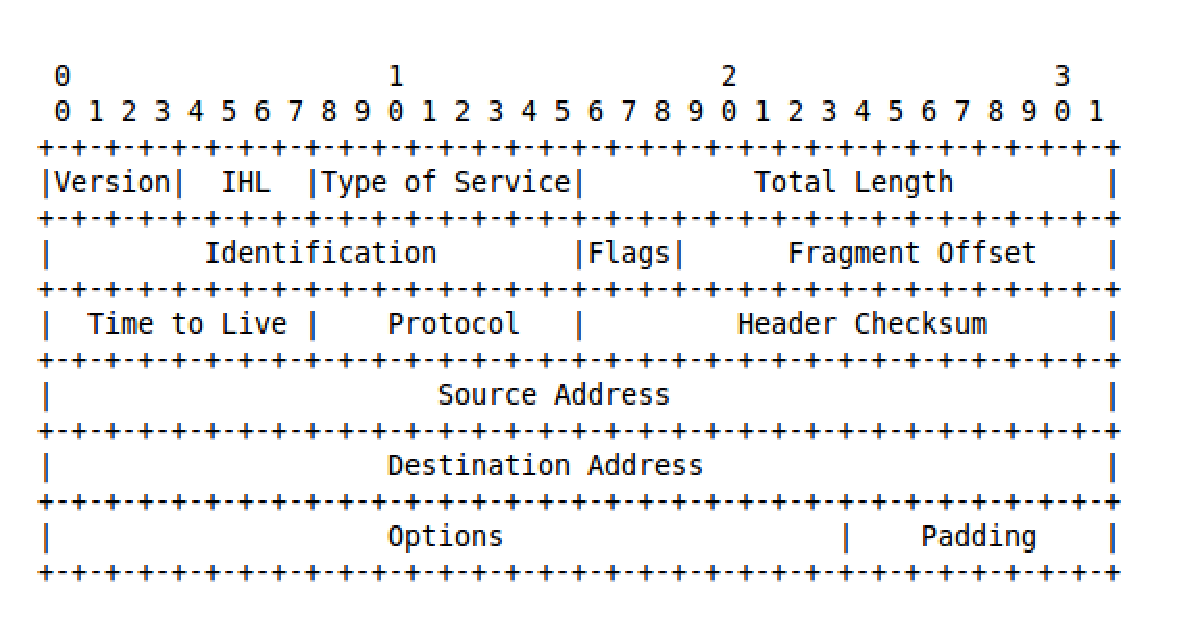
\includegraphics[width=15cm]{./pics/IPv4header.eps}


Comme on peut voir dans la figure ci dessus, un en-tete IPv4 est compose` par
13 champs. En realite nous verrons plus loin que cet en-tete peut, quand il est
necessaire, contenir un champ additionel qui servira a specifier quelque
option qui n'est pas presente dans le 13 champs ci dessus.


Commencons par voir plus en detail les 13 champs d'un en-tete IPv4 standard:

\begin{description}
\item [Version] 
Cette champ occupe les premiers 4 bits de l'en-tete IPv4. Il est
utilise pour determiner le type de protocole utilise` par la couche
reseau (chouche 3). Dans le cas de IPv4 cet champs contiendra toujours
la valeur 4, qui justement identifie le protocole IPv4.

La position de ce champ dans l'en-tete n'est pas casuelle. En effet pour
connaitre la positions des autres champs de l'en-tete il faut d'abord savoir
quel est le protocole utilise et donc le type de en-tete.
En pratique dans la plus part des cas cet champ n'est pas tres utile, car le
protocole a utiliser pour la couche 3 est souvent specifie dans l'en-tete du
protocol de la couche liason.

\item [IHL]
Le champ IHL specifie la taille de l'en-tete IPv4, en fait IHL est 
l'acronime de Interet Header Length. Bien entendu, en disant cela on souligne
un concept important a propos du protocole IPv4: la taille de l'en-tete n'est pas fixe.

La taille de l'en-tete est exprime`e en bloques de 32 bits. Etant donne une taille de
4 bits pour le champ IHL, la longueur maximale d'un en-tete IPv4 est de 15 bloques de
32 bits, qui correspond a 60 octets. Comme l'en-tete IPv4 a une taille minimale
de 20 octets (160 bits), le champ IHL ne peut pas contenir un valeur inferieure a 5.

\item [Type of Service]
Le champ Type of Service, mieux connu avec l'acronime ToS, est utilise pour 
specifier la qualite de service souhaite pour l'envoi d'un packet IPv4.
Cet champ occupe un octet de l'en-tete et il se compose en trois parties.
Une premiere partie de 3 bits permet d'indiquer la precedence avec la quelle
le packet doit etre traite, les 3 bits apres sont utilise pour specifier 
certaines caracteristiques du service, notament: le temp, le debit et la fiabilite.
Enfin l'emploi des 2 derniers bits n'a pas ete specifie et leur usage a ete 
laisse libre pour des implementationes futures.


En realite l'histoire de cet champs est bien plus longue et complexe que ca,
car en pratique la facon d'utiliser cet champs a ete modifie plusieurs fois au 
cours des annees.
\footnote{L'utilisation des 8 bits du champ ToS a ete redefinie
par cinq standard differents (plus divers standars experimentals).
Les documents presentent ces standard sont mentionne dans le chapitre 
"Historical Definitions for the IPv4 TOS Octet" du RFC 3168}
Cette manque de stabilite a par fois cause une certaine confusion dans les implementations.
\footnote{Comme le souligne le RFC 3260 {\it "At least one implementor has expressed confusion about the
relationship of the DSField, as defined in RFC 2474, to the use of
the TOS bits, as described in RFC 1349"}}

Aujourd'hui les 8 bits du champ ToS sont utilise par le mecanisme DiffServ
(Differentiated Services). Cet systeme utilise les premieres 6 bits du champ
ToS (DSCP - Differentiated Services Code Point) pour marquer chaque paquet
comme appartenant a un niveau de priorite et une classe de service.  Chaque
classe determine le type de traitement que on souhaite demander pour le paquet
aux routers au long du chemin (PHB - Per-Hop behaviour), toutefois le service offert
par chaque router est fortement lie a sa configuration.
\footnote {
{\it "The DiffServ standard does not specify a precise definition of "low," "medium,"
and "high" drop probability. Not all devices recognize the DiffServ (DS2 and
DS1) settings; and even when these settings are recognized, they do not
necessarily trigger the same PHB forwarding action at each network node. Each
node implements its own response based on how it is configured."} - 
Implementing Quality of Service Policies with DSCP
http://www.cisco.com/c/en/us/support/docs/quality-of-service-qos/qos-packet-marking/10103-dscpvalues.html
}}
Le dernieres 2 bits du champ ToS sont utilise pour l'extension ECN ({\it Explicit Congestion
Notification }). Cette extension, propose par RFC2481 et introduite deux annees apres avec le RFC3168,
ajoute un systeme de controle de la congestion du traffic reseau. Dans le cas d'une saturation
de la reseau cet champ est utilise pour notifier cet probleme et demander a le dispositif emetteur
une reduction du rythme au quel les packets sont envoye, avec l'objectif de reduir l'attente et
la perte de packets.

\item [Total length]
Comme le suggere le nom, ce champs est utilise pour indiquer la taille totale du
packet IPv4: en tete plus donnes. Le champ {\it Total length} est defini sur 16
bits, ceci permet de indiquer un valeur compri entre 0 et 65,535 octets. Comme l'en-tete
est compris dans la longeur totale d'un packet cet valeur ne sarait jamais inferieur
a 20 (taille minimale d'un en-tete IPv4 en octets).
RFC 791 impose a toutes les dispositifs d'une reseau IPv4 la capacite de recevoir
des packets jusq'a une taille de 576 octets, cette prerogative permet de
eviter une excessive fragmentation.

\item [Identification]
Cet en-tete (sur 16 bits) permet d'identifier les fragments appartenent au meme packet.

\item [Flags]
Le 3 bits du champs Flags sont utilise pour gerer la fragmentation d'un packet.
Un de ces bit est emploie pour indiquer si le paquet peut etre fragmente ou
non. Cet bit, appelle DF ({\it Don't Fragment}), doit etre pris en consideration
par les routers dans le chemin pour decider si un paquet trop grand pour etre
trasmis peut etre retrasmis sous forme de fragments plus petits ou rejete. 
Un autre bit, appelle MF ({\it More Fragments}), indique si le paquet est suivi 
par d'autres fragments. Le bit MF est mis a 0 dans le dernier fragment ou dans
des paquet qui n'ont pas ete fragmente.

Un des trois bits de ce champs n'est pas actuallement utilise mais il a ete
reserve pour applications futures possibles.
\footnote {Cet bit a ete aussi le protagoniste d'un des plus connu poissons
d'avril presentee par le IETF. Pour faciliter les taches des systems de filtrage 
le RFC 3514 propose d'utiliser ce bit pour etiqueter paquets mailveillant, a ce
titre tous les paquets etant envoye avec ce bit (renomme "{\it Evil Bit}") 
mis a 1 seront mis a la poubelle.
}

\item [Fragment Offset]
Lorsque un paquet a ete fragmentee cet en-tete est utilisee pour determiner la 
position (offset) d'un fragment par rapport a les donnees du paquet reassemble.
Le decalage de chaque fragment est exprime en bloques de huit octets (ou 64
bits).  Le champ Fragment Offset utilise 13 bits de l'en-tete IPv4, cela permet
un offset maximale de 65,528 octets.\footnote {En pratique un tel offset n'est
jamais utilisee car, en ajoutant un en-tete minimale de 20 octets, la taille 
totale du paquet reassemble depaserait la longeur maximale d'un paquet IPv4.}
Etant donne que la flag MF ({\it More Fragments}) doit etre mise a zero lorsque 
si un paquet n'est pas fragmentee ou si il est le dernier fragment d'un paquet
plus grand, l'unique difference entre ce deux types de paquets est le valeur
de le champ Fragement Offset que, dans le cas d'un paquet pas fragmentee, est
toujours zero.

\item [Time to Live]
Cet champ determine le nombre maximal de fois qu'un paquet peut etre retrasmis, 
il est utilise pour empecher que un paquet puisse etre retrasmis a l'infini.
Chaque router au long du chemin d'un paquet est tenu a detruir un paquet si le
valeur du TTL ({\it Time to Live}) est zero ou decrementer cet champs par le
nombre de secondes que le paquet passe en attente d'etre trasmis.

En theorie le TTL indique le nombre de secondes pendant le quels un paquet
peut continuer a etre retrasmis dans une reseau ,mais , etant chaque router
toujour tenu a decrementer cet champ de au moins 1 (meme si le paquet a ete
retrasmis en moin qu'un seconde) et considerant les performances des routers
d'aujourd'hui, en pratique le TTL indique le nombre maximum de router que
un paquet peut incontrer au long de son chemim.

Le space reservee au TTL dans l'en-tete IPv4 est de un octet ce que comporte un 
TTL maximum de 255.\footnote {Le RFC 1700 recommende un valeur par defaut de 64.}

Quand un paquet a ete detruit ensuite a l'expiration du TTL, le router qui a
detruit le paquet peut decider de envoier un message d'erreur a l'emetteur du
paquet detruit. Cet type de message (ICMP Time exceeded) est utilise par
utils comme {\it traceroute} pour decouvrir, approximativement, le chemin 
d'un packet IP.

\item [Protocol]
Chaque paquet IPv4 specifie le protocole utilise par les donnes trasmises:
cela est l'objectif de ce champs de 8 bits 

\item [Header Checksum]
Cet champ contient une somme de controle et est utilise pour detecter des 
erreurs dans l'en-tete IPv4. Le valeur de cet champs est recalcule at
chaque retrasmission\footnote {Cela est necessaire car le TTL est decrementee
at chaque retrasmission et un changement de l'en-tete comporte un valeur different
dans la somme de controlle}: si il ne correspond pas avec celui 
presente dans l'en-tete le paquet est detruit.


\item [Addresse source et Addresse destination]
Les addresses de chaque paquet IPv4 (soit l'adresse source que l'adresse de
destination d'un paquet) sont represente sous forme d'une suite de 32 bits.

L'addresse source de chaque packet represente dans la plus part des cas
l'addresse logique\footnote {Il ne faut surtout pas oublier la difference entre
un addresse physique, comme par example un addresse MAC (qui est lie a
l'hardware et est donc unique pour chaque machine), et un addresse logique,
comme par example un addresse IP (qui peut changer et identifie une machine
dans une reseau en particuliere).} de la machine qui a envoye le paquet
(a laquelle il faudra eventuellement repondre donc).  Dans certains cas
specifiques cette addresse ne correspond pas a celui de la machine qui a envoye
le paquet, c'est par exemple ce qui se passe dans une requete {\it ARP probe}
la ou le valeur de l'adresse de la machine source est 0.0.0.0 (ce qui represente
un adresse indefini\footnote {Notex que la signification de l'adresse 0.0.0.0
est lie a la facon dont il est utilise. En general il indique {\it aucune
adresse en particulier}.  Dans la plus part des cas cet adresse est utilise
pour indiquer un de ces valeurs: l'adresse de la machine courant (c'est
l'adresse de loopback), n'importe quel adresse ou reseau (c'est le cas de la
route par default dans une table de routage), un adresse indefini ou bien une
combinaison des possibilites precedentes (c'est le cas d'une requete {\it ARP
probe} ou bien d'une requete {\it DHCP Discovery} ou {\it DHCP Request}, ou en
fait l'adresse source 0.0.0.0 indique un adresse indefinie mais aussi l'adresse
de la machine actuelle, que del reste n'est pas encore defini...).}
) car elle n'a pas encore determine son addresse IP. 

L'addresse de destination d'un paquet IPv4 identifie la machine vers
laquelle le paquet doit etre expedie. Comme dans le cas de l'adresse source,
aussi l'adresse destination peut contenir des valeur speciaux. En effet certains 
valeurs puvent etre utilise par example pour identifier plusieurs machines
(adresses multicast), toutes le machines d'une reseau (adresse de broadcast) ou
la machine actuelle (adresse de loopback).

Une description plus detaile des mechanismes lies aux adresses IPv4 est
propose dans le chapitre 
%TODO mettre chapitre% 
de ce rapport.


\item [Options] 
Cet champ n'est pas obligatoire et donc il peut ne pas etre present dans un
en-tete IPv4. La presence de cet champ est determine par le valeur du
IHL: lorsque cette valeur indique une taille de l'en-tete IPv4 superieure a 
la taille minimale (20 octets), l'en-tete contiens des options.
Etant donne que un en-tete IPv4 peut avoir une taille maximale de 
60 octets (le valeur du IHL est egal a 15), le champ Options peut occuper
40 octets au meximum.

Ce champ est ne pour etendre les possibilites de IPv4 en ajoutant des fonctions extra.
Aujord'hui il y a quelque dizaine de options qui ont ete specifie\footnote
{http://www.iana.org/assignments/ip-parameters/ip-parameters.xhtml} (si on
considere aussi les options experimentales) mais peu entre eux sont reelement
utilise. 
Entre les options les plus connues on retrouve par example des ajoutes
utiles a l'administration et au debouggage d'une reseau, comme {\it Record route}
qui permet de enregistrer les addresses des routeurs dans le chemin d'un 
paquet IP, et {\it Timestamp} qui permet de savoir le temp passe 
entre chaque hop du chemin.

Entre les options il en y a deux qui ont une fonction speciale: EOL 
({\it End Of Option List}) and NOP ({\it No Operation}): l'option EOL 
est utilise pour indiquer la fin de la chaine d'options, NOP est une option
sans aucun effet, elle est utilise comme replissage pour aligner les options 
quand elles ne sont pas aligne sur 4 octets\footnote {On rappelle que 
le champ IHL indique la longuer de l'en-tete IPv4 en bloques de 32 bits 
(4 octets)}.



\item [Padding] 
Le padding ne contiens que des zeros et est utilise quand la fin de l'en-tete
n'est pas aligne sur 32 bits (4 octets). Bien entendu, cet champ est optionel:
en effet il pest etre necessaire seulement lorsque l'en-tete IPv4 termine avec
une option lequel limite n'est pas aligne sur 32 bits. Un en-tete n'a besoin
d'aucun Padding standard IPv4 de 20 octets (donc sans aucune option) termine
comme etant aligne sur 4 octets (20 est un multiple de 4).



















\end{description}



%Victor
\section{Suite de protocole}

\subsection{ARP}
ARP (Address resolution protocol) est un protocole à cheval sur la couche 2 et
la couche 3. La fonction principale d'ARP est de faire la conversion entre les
adresses de niveau 2 et de niveau 3. Cela est très utilisé étant donné que les
hôte connaissent souvent les adresses IP de leur destinataire, mais rarement
l'adresse de niveau 2 de ce destinataire ou de la passerelle à contacter pour joindre
le destinataire.

\subsubsection{Exemple}
Dans la partie qui suit nous allons nous placer dans l'exemple suivant.
TODO LAN exemple
\subsubsection{Entête}

\subsubsection{Fonctionnement}
Prenons l'exemple où A veux envoyer un message à B. A connait l'adresse IP de
B. Donc A va préparer son paquet qu'il va envoyer à B, avec son adresse IP en
source et l'adresse IP de B en destination. La paquet passe dans la couche
liaison, il va être enpaqueté dans une trame de niveau 2. Cette trame aura
comme adresse source l'adresse de niveau 2 de A, mais à ce moment il ne peux
pas completé l'adresse destination de la trame: en effet, il ne connait
l'adresse de niveau 2 du destinataire. La paquet reste bloqué en couche 2 et ne
peux pas être envoyé au destinataire. Comment obtenir l'adresse de niveau 2 du destinaire?
Le protocole ARP est capable de faire cette translation.

\subsubsection{ACD}
Adresse conflict detection
\subsection{ICMP}
ICMP (Internet Control Message Protocol) est un protocole de niveau 3 faisant partie intégrante du protocole IPv4. Il permet de transmettre des informations de controle et d'erreur. Les messages ICMP sont empaquetés dans des paquets IP, ils diposent donc d'un entête de paquet IP. Cet entête est le même que pour tout les autres entêtes de paquet d'IPv4. Deux champs son intéressant dans le cas d'un paquet ICMP, les champs Protocol et Type of service. Le champ Protocol est mis à à la valeur 1 pour dire que le paquet contient un message ICMP, et le champ ToS est mis à 0 //TODO(pourquoi 0?)//.
Après le header du paquet IPv4, commence la partie data qui contient le message ICMP. Ce message contient des champs différent en fonction du type de message à passer. Cependant les trois premier champs sont toujours les mêmes.
Les types de messages ICMP qui vont suivrent sont décrit dans la RFC 792.\footnote{https://tools.ietf.org/html/rfc792}
\\
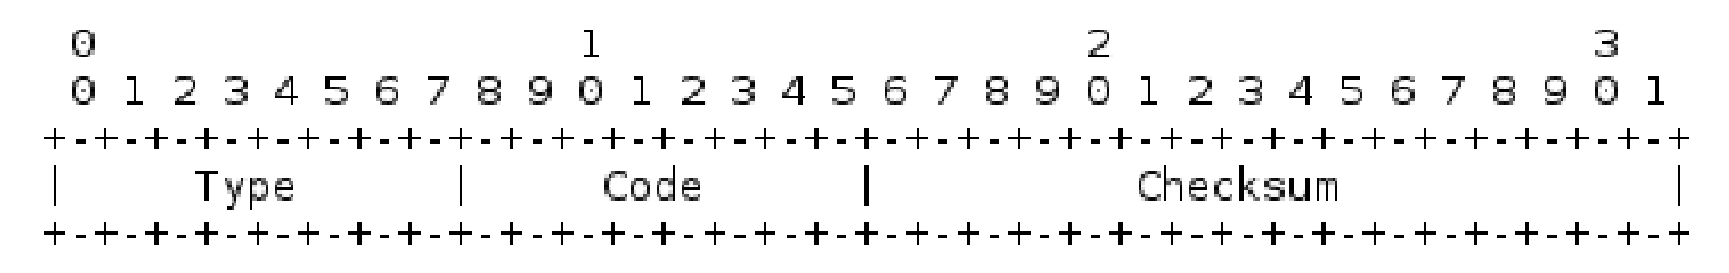
\includegraphics[width=15cm]{./pics/header.eps}
\\Le premier champ est celui de type. Il permet, premièrement, de donner le type du paquet et de l'information à transmettre, et deuxièmement de préciser la nature des champs qui vont suivres. En effet, comme vu plus haut, les messages contiennent des champs différents selon le type du message ICMP.
\\Le deuxième champ est le code. Il permet de subdiviser le type en donnant des détails plus précis.
\\Enfin le troisième champ est la somme de contrôle (checksum)//TODO(plage de controle).
\\Commençons avec les messages qui possèdent l'ensemble de champs le plus simple.

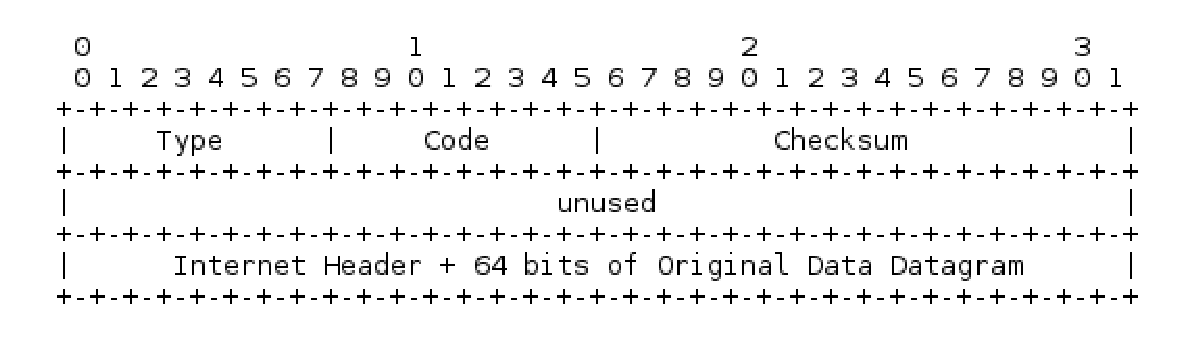
\includegraphics[width=15cm]{./pics/header1.eps}

\\Les messages qui utilisent cette organisation sont les messages de type 3, 4 et 11.

\subsubsection{Message de type 3: Unreachable Destination}
Les messages de type 3 sont émis lorsqu'un paquet n'a pas réussi à joindre la destination (Unreachable destination). Cette erreur peux être dut à plusieurs facteurs, et les codes permettent de préciser pourquoi le paquet n'a pas pu rejoindre sa destination.
\paragraph{Code 0}

\subsubsection{Message de type 4:}

\subsubsection{Message de type 11: Time Exceeded}
Ces messages sont envoyés lorsque le TTL d'un paquet à atteind 0. Une autre utilisation des ces messages est lorsque que le temps de ré-assemblage des fragments d'un paquet est dépassé. Ces deux cas sont distingé par le code. Ces messages ont pour destinataire l'hôte qui à envoyé le paquet qui à provoqué l'erreur.//TODO(vérifier)
Le champ Internet header contient l'entête du paquet qui a été supprimé plus les 64 bits suivant celui-ci. Cela permet à l'émetteur de retrouver quel paquet à été supprimé.
\paragraph{Code 0:}
Le code 0 est utilisé pour indiquer que le TTL du paquet posant problème est arrivé à 0. Lorsque le TTL d'un paquet arrive à 0, celui-ci est supprimer et un message ICMP de type 11 et de code 0 est envoyer par le routeur qui à détécté le problème. Cela permet principalement d'éviter qu'un paquet sans dans une boucle et qu'il soit rélayé à l'infini.
\paragraph{Code 1:}
Le code 1 est quant à lui utilisé pour indiquer //TODO


\subsubsection{Message de type 5:}
Les message de type 5 utilisent les entêtes ci-dessous et servent à faire de la redirection. En effet, lorsqu'un routeur détecte que le prochain routeur dans lequel va transiter le paquet se trouve dans le même réseau que l'émetteur de ce paquet, il va envoyer un message ICMP pour avertir cet hôte (et/ou le réseau) qu'il existe un chemin plus court en envoyant directement les paquets vers le prochain routeur. Ce message ICMP va avoir pour effet de modifier la table de routage interne à l'émetteur (et/ou des hôtes connecté au réseau). Concernant le paquet que le premier routeur à reçu, il va le transmettre vers sa destination.

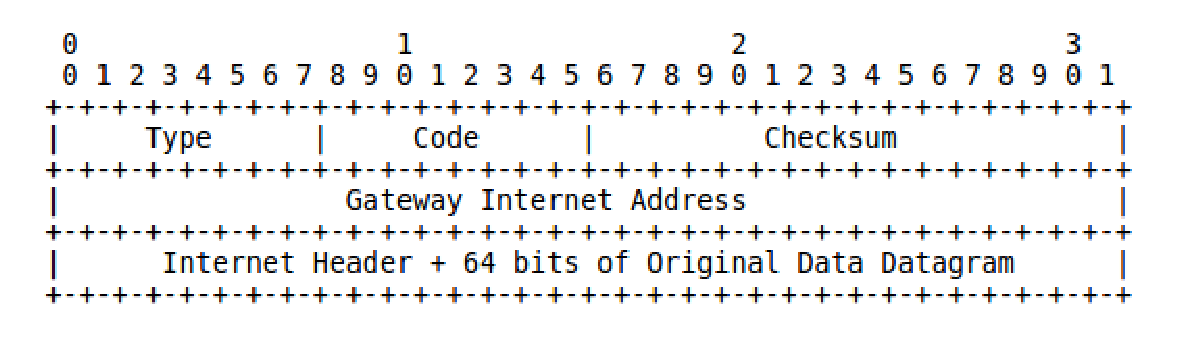
\includegraphics[width=15cm]{./pics/header2.eps}

\\
Le champ Gateway Internet Address contient la l'adresse du routeur auquel il faut faire transiter le traffique directement pour avoir un chemin de routage plus court.
Le champ Internet Header contient toujours l'entête du message ayant porvoqué l'envoie du message ICMP plus les 64 bits suivant l'entête. Cela permet à (aux) hôte(s) de pouvoir modifier leur table de routage en fonction la destination que cherchait à atteindre le paquet.
\paragraph{Code 0}
Ce code indique que la redirection est adresser à tout le réseau de l'émetteur du paquet.
\paragraph{Code 1}
Ce code indique que la redirection est adresser à l'émetteur du paquet.
\paragraph{Code 2}
Ce code indique que la redirection est adresser à tout le réseau de l'émetteur du paquet et aux services(//TODO(préciser)).
\paragraph{Code 3}
Ce code indique que la redirection est adresser à l'émetteur du paquet(//TODO(préciser)).

\\
\\
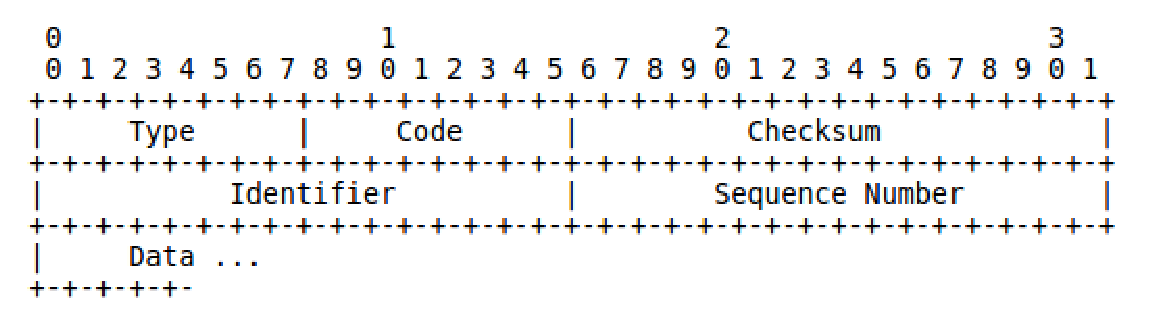
\includegraphics[width=15cm]{./pics/header3.eps}
\\

\subsubsection{Message de type 8 et 0:}
Les messages de type 8 et 0 servent à faire des envoies et des renvoies d'information. Ils utilisent pour cela l'entête ci-dessus. Les messages de type 8 font des envoies d'informations, appelé echo request. Tandis que les messages de type 0 sont envoyés en réponse aux echo request et renvoie les informations reçus de ceux-ci; ils sont appelés echo reply. Etant donnée que les echo reply sont des réponses aux echo request, l'adresse destination des echo reply est l'adresse source des echo request. Ces deux messages peuvent envoyés et reçu aussi bien par un hôte que par un routeur. Ce sont notamment les message envoyés par la commande {\it ping} qui permet de vérifier si l'on peux communiquer avec un hôte ou un routeur.
Les champs Identifier et Sequence Number aide l'émetteur de l'echo request à associer les echos request qu'il à envoyés avec les echos reply qu'il à reçus.
//TODO(qui a t-il dans data?)
\subsection{IGMP}


\subsection{DHCP}
\footnote{RFC 2131: https://tools.ietf.org/html/rfc2131}
Le protocole DHCP (Dynamic Host Configuration Protocol) sert à l'autoconfiguration des interfaces. Plus précisement, il  permet d'attribuer une adresse IP à une interface et de lui faire parvenir d'autres information essentielle pour le fonctionnement de l'interface sur le réseau.
Voyons comment une interface peut ce configurer aurpès d'un serveur DHCP.

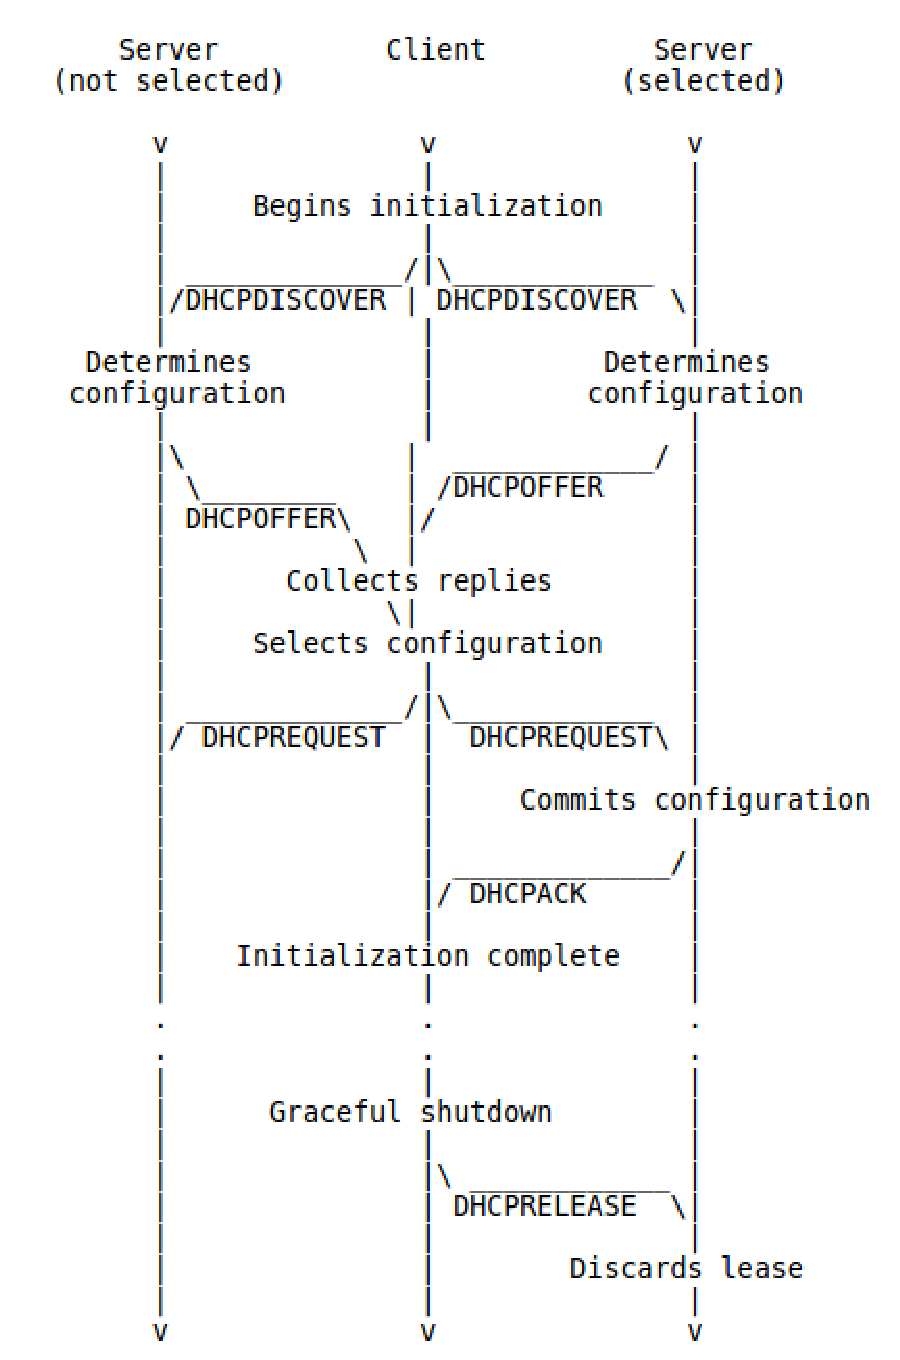
\includegraphics[width=6cm]{./pics/timeline_dhcp.eps}
\\
Lorsqu'une interface, qui n'a pas d'adresse IP, souhaite en recevoir une, elle va emettre un message DHCPDISCOVER en broadcast sur son réseau. Des agents DHCP peuvent faire passer ce message DHCP sur un autre réseau si le serveur DHCP (qui distribue les adresses) ne se trouve pas sur le même réseau que l'hôte qui fait la demande. L'hote va utiliser comme adresse IP 0.0.0.0.
\\Etant donnée que le message est envoyé en broadcast, tout les hôtes sur le réseau vont recevoir le message, et en particulier le ou les serveurs DHCP qui pourraient s'y trouver. Si cela est le cas, ceux-ci vont répondre avec un DHCPOFFER. Ce message contient entre autre l'adresse IP proposé pour le client souhaitant se configurer, ainsi que le masque de sous-réseau de l'adresse. A ce moment là l'adresse n'est pas encore attribuer et réservé pour l'hôte étant donnée qu'il peux refuser l'offre et accepter l'offre d'un autre serveur. Si jamais l'hôte ne reçoit aucun DHCPOFFER, il va ré-émettre un DHCPDISCOVERY. Si il reçoit un ou plusieurs DHCPOFFER, l'hôte va devoir choisir une configuration qui lui est proposé. Une fois ce choix fait, il va informé les serveurs DHCP de son choix à l'aide d'un message DHCPREQUEST émis en broadcast. Ce message va contenir l'identifiant du serveur DHCP retenu ainsi que la configuration souhaité par l'hôte (adresse IP et masque de sous-réseau). Ce message peut être interprété de deux manières différentes selon le serveur:
\item- si ce n'est pas le serveur retenu, il considère le message comme une déclinaison de l'offre.
\item- si c'est le serveur retenu, il va sortir l'adresse attribué l'hôte de la plage d'adresse libre pour ne plus l'attribuer à un autre hôte. Il va ensuite émmetre un message DHCPACK contenant la configuration effective de l'hôte avec notemment: l'adresse IP, le masque de sous-réseau, la durée du bail, l'adresse de la passerelle par défaut et l'adresse du serveur DNS.
Si pour quelque raisons le serveur n'est pas capable d'attribuer l'adresse proposé dans l'offre (par exemple si l'adresse à été attribuer entre temps), le serveur emet un DHCPNAK pour avertir l'hôte que l'adresse n'est plus disponible. L'hôte devra alors recommencer la procédure pour obtenir une adresse IP.
\\Enfin si le serveur ne reçoit pas de message DHCPREQUEST, la procédure s'arrêtrra à ce moment et l'adresse n'étant pas encore attribuer à l'hôte elle reste disponible pour être attribuer à d'autre hôte.
Arrive la dernière étape. Si le client reçois un message DHCPACK, il peux prendre en compte la configuration (adresse IP, masque de sous-réseau, DNS, passerelle par défaut et durée de bail). Il va effectuer une dernière vérification pour s'assurer que l'adresse qui lui à été attribué est bien unique sur le réseau pour éviter d'avoir deux hôte avec la même adresse. Il va pour cela utilisé le protocole ARP et la méthode de vérification vu plus haut. Si jamais l'adresse est déjà utilisé par un autre hôte, il va envoyer un message DHCPDECLINE au serveur DHCP pour lui indiquer qu'il n'utilisera pas la configuration proposé par celui-ci, et il va recommencer la procédure pour pouvoir obtenir une nouvelle configuration.
\\Si jamais l'adresse proposé par le serveur est unique sur le réseau, la configuration est terminé et l'hôte peut utiliser l'adresse (durant la durée du bail de celle-ci).
Dernier cas possible, si jamais le l'hôte ne reçoit pas de DHCPACK ou de DHCPNAK, il va réemettre le message DHCPREQUEST pour esperer recevoir une réponse du serveur.

//TODO algo de retransmission
//TODO fonctionnement agent relais dhcp
//client peut renoncer à son bail
//identification des message faisant partit d'un meme echange avec client identifier, server identifier
//TODO fonctionnement bail

L'hôte est donc configuré et peut utiliser son adresse. Cependant, il ne peut l'utiliser que durant la durée de son bail. Une fois le bail expiré, l'hôte ne peux plus utiliser son adresse. Lorsque l'hôte à reçu le message DHCPACK du serveur, celui-ci lui a transsmis la durée du bail. De cette durée, l'hôte va en extraire deux temps noté T1 et T2. T1 correspond à la moitié de la durée du bail et T2 à 0.875 la durée du bail. Ces temps sont exprimé de manière relatif étant donnée que les horloges du serveur et de l'hôte ne sont pas synchronisées.
Une fois que l'hôte à atteind le temps T1, il va chercher à contacter le serveur qui lui à attribué sa configuration avec un message DHCPREQUEST pour étendre la durée de son bail. Ce message est émis de manière unicast. A ce moment l'hôte est entré en état RENEWING. Si l'hôte reçoit un message DHCPACK du serveur lui accordant un prolongement de la durée de son bail, alors il va sommer le temps qu'il avait insérer dans le DHCPREQUEST avec la durée accordé par le serveur et qui se trouve dans le message DHCPACK. L'hôte retourne dans l'état BOUND. Cependant l'hôte n'est pas obligé d'attendre T1 pour pouvoir étendre son bail.
Si jamais l'hôte ne reçoit pas de reponse DHCPACK avant l'arrivé de T2, il passe en état REBINDING. A ce moment il va émettre un DHCPREQUEST en broadcast pour espérer pourvoir étendre son bail auprès de n'importe quel serveur DHCP. Pour parer aux eventuels cas de perte de DHCPREQUEST, l'hôte va renvoyer un message une fois la moitié de la durée entre T1 et T2 passé, en état RENEWING; et une fois la moitié de la durée entre T2 et la fin du baille , en état REBINDING(et avec un minimum de temps de 60 secondes).
Si malgré tout, la durée du bail venait à expirer, alors l'hôte ne possèderait plus de configuration réseau et ne pourrait plus communiquer avec d'autre hôtes. Il rentre alors en état INIT; il doit alors recommencer la procédure pour obtenir une adresse configuration.

Cependant,dans ce cas comme dans d'autre, l'hôte peut ré-utiliser une configuration précédement utilisée. Cela permet de raccourcir la négociation entre l'hôte et le serveur DHCP. L'hôte va directement commencé la négociation en faisant un DHCPREQUEST en broadcast et contenant la configuration qu'il souhaite ré-utiliser. Le serveur concerné par l'attribution antérieur de la configuration va donc accepter la demande de l'hôte à l'aide d'un DHCPACK ou la refuser, si la demande n'est pas correct ou si l'adresse est utilisé par un autre hôte, à l'aide d'un DHCPNAK.
Cette négociation se fait de manière similaire qu'un négocation complète, elle a juste été raccourci en enlevant quelque étape non indispensable.

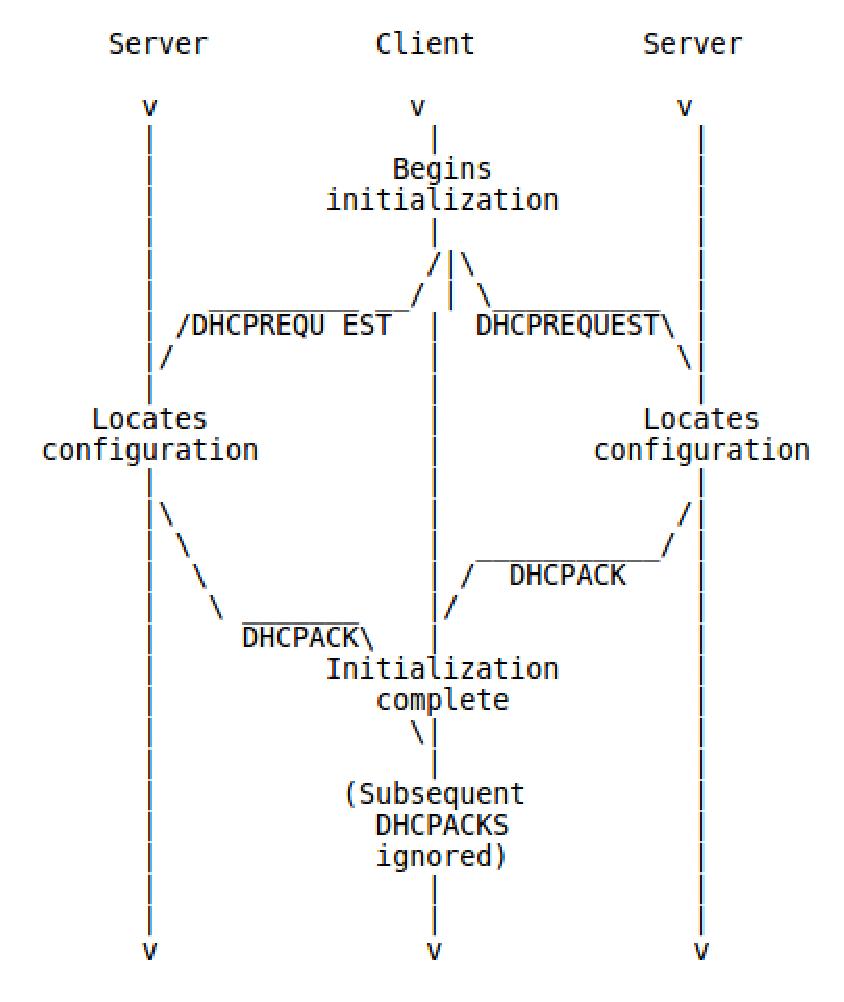
\includegraphics[width=6cm]{./pics/timeline_dhcp_reuse_add.eps}


\section{Passage de IPv4 à IPv6}
\subsection{Raison du passage de IPv4 à IPv6}
\subsubsection{Problème posé par IPv4}
//Pénrurie, adressage privé/publique compliqué
% Il se trouve que apparement il y a des problemes de
% penurie d'adresses meme dans certaines reseau prive`
% http://blog.erratasec.com/2013/12/dod-address-space-its-not-conspiracy.html#.WAf_d7Wf21F

PROBLÈMES DE IPV4

ÉPUISEMENT DES ADRESSES
Lorsque IPV4 a été développé dans les années 70-début des années 80, personnes n'aurait imaginé qu'il y aurait un jour autant d'interfaces qui se connectent à Internet. On pensait qu'une adresse sur 32 bits serait suffisante. De plus, les plages d'adresses étaient distribuées généreusement au début. Cela veut dire que l'on attribuait des adresses permettant un nombre d'interfaces beaucoup plus grand que nécessaire.
Cependant, avec la croissance du nombre d'utilisateurs, la plage d'adresses IPV4 disponible a diminué progressivement. C'est en février 2011 que la réserve de bloc libres d'adresses publics IPV4 de l'IANA (Internet Assigned Numbers Authority) est arrivée à épuisement.
Afin de résoudre ce problème, plusieurs techniques ont été proposées.
La première a été le changement de teechnique d'adressage. On est passé de la technique de classe d'adressage IP à la technique Classless Inter-Domain Routing. Ceci à permis une meilleure efficacité dans la distribution des adresses IP grâce à la création de réseau de tailles intermédiaire. En effet, avant on ne disposait que de réseau de 3 tailles différentes.
Les politiques d'assignement d'adresses ont également été rendu plus stricte afin de mieux tenir compte des besoin réels des demandeurs d'adresses IP.
Il a aussi été décidé d'utiliser des blocs autrefois réservé comme 14.0.0.0.
Sur base de volontarisme, des blocs autrefois attribués généreusement ou alors des IP non utilisées ont été récupérées. 
Finalement, il a été remarqué qu'il n'était pas nécessaire que chaque interface a son adresse IP public et le protocole NAT a été développé afin de regrouper plusieurs interface sous une même adresse IP. Ce protocole est de plus en plus utilisé dans IPV4 depuis la fin des années 90.

Fonctionnement du NAT dynamique (Network Adress Translation)
Le NAT est une technique utilisée au niveau du routeur. Le principe du NAT est que le routeur fait correspondre à une adresse IP une autre adresse IP. En général cette technique est utilisée pour avoir une même adresse IP pour tout un réseau comme un intranet ou encore un réseau domestique. Dans ce réseau, toutes les interfaces - même le routeur - auront une adresse privée. Le routeur dispose en plus de cela de une ou plusieurs adresses publics avec lesquelles il est connecté à internet. Une adresse privée est une adresse qui est utilisée à l'intérieur d'un réseau local. Les adresses privées peuvent être choisies parmi les suivantes : 10.0.0.0/8, 172.16.0.0/12 ou 192.168.0.0/16.
Lorsqu'une interface envoie un paquet vers l'extérieur du réseau, le routeur effectue plusieurs changements. Il traduit d'abord l'adresse privée en adresse public et la met dans l'en-tête du paquet. Puis il change tous les checksums qui tiennent compte de l'adresse IP. Enfin, il garde en mémoire dans une table la correspondance entre adresse privée/adresse public comme ci-dessous.
<tableau adresse public / privée >
Cela n'est cependant pas suffisant. En effet, lorsqu'un paquet arrivera de l'extérieur du réseau,  et si tous les interfaces utilisent la même adresse public sans distinction supplémentaire, le routeur ne saura pas à quelle interface envoyer le paquet. 
Une solution à ce problème existe pour les protocoles utilisant les ports comme TCP et UDP. Le routeur ajoute une information supplémentaire dans la table qui est le port source d'où vient le paquet. Les ports, qui sont implémentés dans la couche transport (couche 4), sont des sortes de ''portes'' qui permettent de communiquer avec un système d'exploitation. Le numéro de port est un numéro choisit aléatoirement entre 1024 et 65535.
Pour illustrer le fonctionnement du NAT imaginons qu'une interface A dont l'ip est 192.168.0.1 veut envoyer un paquet à l'interface B d'ip 217.70.184.38. Le port source est le port 10277 et le port destination est le port 80. 
La table NAT ressemblera à ceci : 

<TABLE NAT complète > 

La box internet enverra le paquet : 

L'interface B répondra en envoyant le paquet :

Lorsque la box reçoit ce paquet, elle voit que le port de destination est le port 10277. Elle cherche ensuite le port correspondant dans sa table NAT. Lorsqu'elle le trouve elle effectue les changements nécessaire sur le paquet et transmet le paquet à l'interface A.
Mais même si cette solution fonctionne la plupart du temps, la probabilité est faible que 2 interfaces envoient des paquet sur les même port. C'est pour éviter cela que la box change le port source lorsqu'elle reçoit un paquet de l'interface A. Ainsi on s'assure que aucun port n'est utilisé plusieurs fois. Enfin, pour éviter de saturer les ports utilisés, un compteur est associé à chaque paire adresse public/adresse privée. Lorsqu'il n'y a pas de trafic entre une adresse privée et l'extérieur durant une durée fixée, le port qui lui est associée peut être réutilisé pour une autre adresse privée.

Le NAT dynamique apporte cependant un grand problème. Lorsqu'une interface extérieur veut se connecter à une interface dans le réseau, elle ne dispose d'aucune autre information que l'adresse IP public. Si elle envoie alors un paquet à cette adresse, le routeur qui le réceptionnera ne saura pas quoi faire avec et le paquet sera perdu. 
 On a réussi à pallier à ce problème grâce au port forwarding. 

PORT FORWARDING

NAT STATIQUE


\subsubsection{Solutions}
//NAT,IPv6
\subsection{Différence entre IPv4 et IPv6}

\section{Conclusion}
\label{sec:ccl}

\addcontentsline{toc}{section}{Références}
\bibliographystyle{plain}
\bibliography{rapport}

\end{document}
